\chapter{PIP project}

\section{PIP protokernel}

\subsection{A minimal OS kernel with provable isolation} \label{PIP}
An operating system is organized as a hierarchy  of layers, each one constructed  upon  the one  below  it. Each layer focuses on an essential role of the operating system such as memory management, multiprogramming, input/output \dots Generally speaking, while developing a kernel for an operating system based on the layered  approach,  the designers have a choice where to draw the kernel-user boundary. Traditionally, all the layers went in the kernel, but that is not necessary. In fact, putting as little as possible in kernel mode is safer because kernel bugs can bring down the system instantly. In contrast, user processes/layers are set up to have less power so that a bug there may not be fatal.\\

Various studies on bug density, relatively to the developed module size, age as well as other factors, have been conducted (e.g.  \textit{Basilli}  and  \textit{Perricone} in 1984;  and \textit{Ostrand}  and  \textit{Weyuker} in 2002). A  ballpark  figure  for  serious industrial systems is ten  bugs per a thousand  lines  of code. Operating  systems  are  sufficiently  buggy  that  computer  manufacturers  put  reset  buttons  on  them, something  the  manufacturers of cars, TV sets and stereos do  not do,  despite  the  large  amount  of software in these devices. Furthermore, Operating systems generally present hardware resources to applications through high-level abstractions such as (virtual) file systems.\\

\noindent Therefore, we can distinguish several OS kernel families such as : 
\begin{itemize}
	\item \textbf{Microkernels :} The basic idea  behind a microkernel design  is  to  achieve high reliability  by  splitting the operating  system  up into small, well-defined  modules, only  one  of  which, the  microkernel, runs  in  kernel  mode;
	\item \textbf{Exokernels :} The idea behind an exokernel is to force as few abstractions as possible on application developers, enabling them to make as many decisions as possible about hardware abstractions.
\end{itemize} 
  
\noindent Although the closest kernel design to PIP is the exokernel, PIP\cite{PIP} does not belong to any of the kernel families featured in the state of art, but it is the first member of a new kernel family, \textbf{protokernels}, as compared to most microkernels and exokernels, the TCB in PIP is even more restricted :
\begin{itemize}
	\item Scheduling and IPC are done in user mode unlike a microkernel;
	\item Multiplexing is also done in user mode unlike an exokernel.
\end{itemize}

\noindent whereas the kernel mode is only for \textbf{multi-level MMU control and configuration} (virtual memory) and \textbf{context switching}. This not only ensures less bugs density but also more feasibility of formal proof that will warrant the memory isolation property of the protokernel. \\

As a \textbf{minimal OS Kernel with provable isolation}\cite{PIPSlides}, PIP focuses more on security and safety without sacrificing efficiency and ensures memory isolation between different tasks running on the same device.PIP's algorithmic part is written in Gallina, the language of the Coq proof assistant, in a monadic style that allows direct translation into free-standing C. We will refer to this implementation in \textit{Gallina} as the shallow embedding in contrast to the deep embedding introduced in section \ref{deep} p.\pageref{deep}. 

\begin{figure}[!ht]
	\centering 
	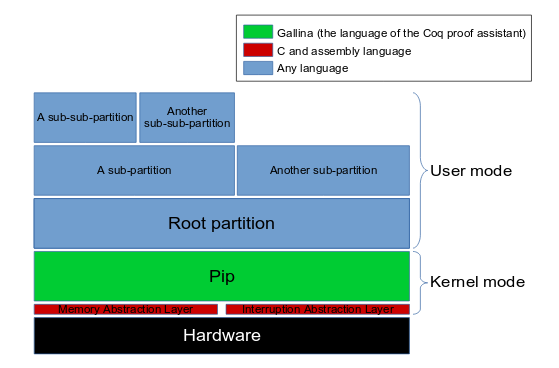
\includegraphics[width=\linewidth ,frame]{img/OSLayersPIP.png} 
	\caption{Software layers of an OS built on top of PIP}
\end{figure}

\subsection{Horizontal isolation \& vertical sharing} \label{properties}

PIP can be used to partition the available memory which will be initially allocated to the root partition on top of PIP. Any partition can read and write in the memory of its children. However, partitions in different branches of the partition tree are disjoint. The former is referred to as \textbf{vertical sharing} and the latter as \textbf{horizontal isolation}. Needless to say, all memory lent to PIP for storing kernel data,such as when creating partitions, is inaccessible for all partitions to prevent messing up PIP data structures which means that the kernel data is totally isolated.
   
\begin{figure}[!ht]
	\centering 
	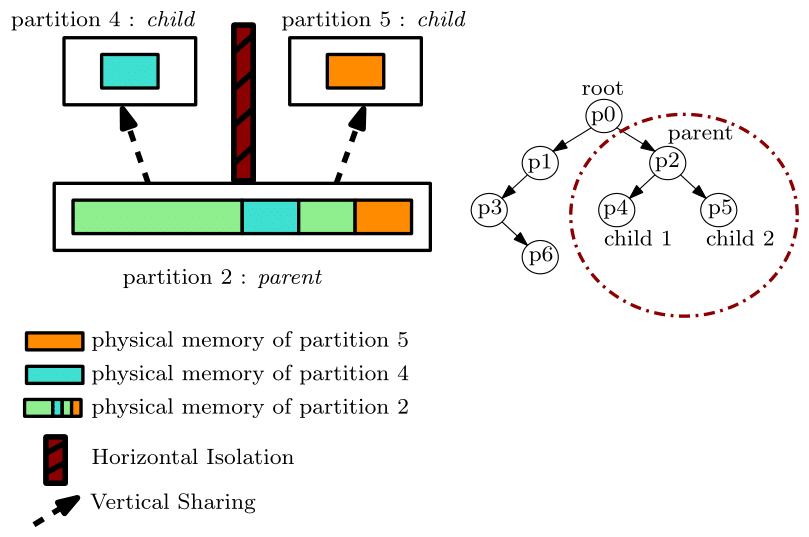
\includegraphics[width=0.8\linewidth,frame]{img/memoryIsolShare.png} 
	\caption{Horizontal isolation \& vertical sharing in PIP}
\end{figure}

\noindent Let us consider a more realistic partition tree, as shown in figure \ref{FreeRTOS}, in which we consider \textit{Linux} and \textit{FreeRTOS} as sub-partitions of a root partition, multiplexer. Knowing that \textit{FreeRTOS} is a real-time OS that does not isolate its tasks, we have easily secured it with task isolation by porting it on PIP.

\begin{figure}[!ht] \label{FreeRTOS}
	\centering 
	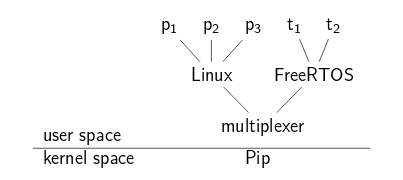
\includegraphics[scale=0.5,frame]{img/FreeRTOSEx.png} 
	\caption{FreeRTOS task isolation using PIP}
\end{figure}

\subsection{Proof-oriented design}

\subsubsection{PIP's design} 
PIP's isolation properties are meant to be formally proven independently from the platform it's running onto. Consequently, the algorithm and the architecture dependant part were separated. Indeed, as shown in figure \ref{design}, PIP is split into two distinct layers  :
\begin{itemize}
	\item \textbf{HAL :} gives direct access to the architecture and hardware;
	\item \textbf{API :} implements the algorithmic part to configure the virtual memory and the hardware.
\end{itemize}

\noindent The API code is written and proven using the Coq proof assistant, and uses the interface provided by the HAL to perform any hardware related operation. the proofs are based on Hoare logic theory introduced in section \ref{Hoare} p.\pageref{Hoare}.

\begin{figure}[!ht]  
	\centering 
	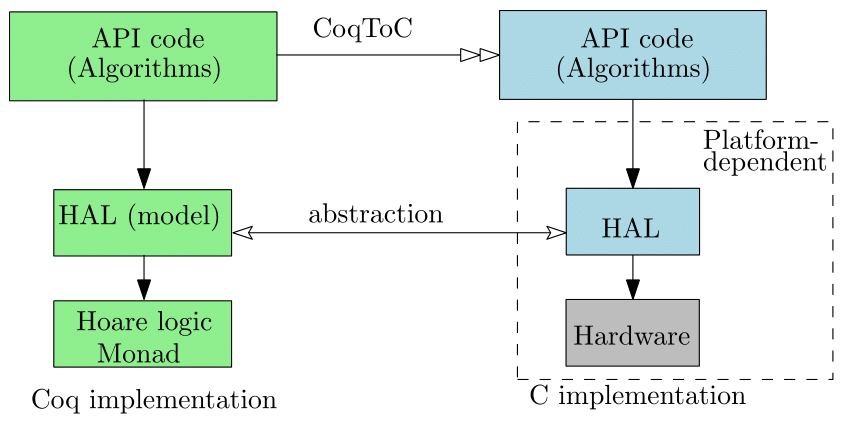
\includegraphics[width=0.8\linewidth, frame]{img/PIPDesign.png} 
	\caption{PIP design}
	\label{design}
\end{figure}

\noindent PIP's HAL is split into three components, as shown in figure \ref{HAL}, each handling a specific part of the target platform's hardware :
\begin{itemize}
	\item \textbf{\gls{MAL} :} provides an interface for the configuration of the MMU chip;
	\item \textbf{\gls{IAL} :} provides an interface to dispatch interrupts and configure hardware;
	\item \textbf{Bootstrap :} contains the low-level code required to boot the system.
\end{itemize}

\noindent PIP only provides system calls for management of the partitions and for context switching, thus reducing the TCB to its bare minimum as explained in section \ref{PIP} p.\pageref{PIP}. This user exposed API can be called by any partition using a platform dependant call :
\begin{itemize}
	\item \textbf{createPartition :} creates a new child (sub-partition) into the current partition;
	\item \textbf{deletePartition :} removes a child partition and puts all its used pages back in the current partition;
	\item \textbf{prepare :} adds required configuration tables into a child partition to map a new virtual address;
	\item \textbf{collect :} removes the empty configuration tables which are not used anymore and gives it back to the current partition; 
	\item \textbf{countToMap :} returns the amount of configuration tables needed to perform a mapping for a given virtual address;
	\item \textbf{addVaddr :} maps a virtual address into the given child;
	\item \textbf{removeVAddr :} removes a given mapping from a given child.
\end{itemize} 
This API is sufficient as far as memory requirements are concerned but it lacks a way to handle interrupts. Hardware interrupts are implicitly handled by PIP and automatically dispatched to the root partition, while software interrupts, such as system calls, are notified to the parent partition of the caller and can be managed by these two additional services of PIP :
\begin{itemize}
	\item \textbf{dispatch :} notifies an interrupt to a given partition, interrupting its current control flow and backing it up for a further resume call;
	\item \textbf{resume :} restores a previously interrupted context.
\end{itemize}
\vspace{-0.8em} 
\begin{figure}[!ht]  
	\centering 	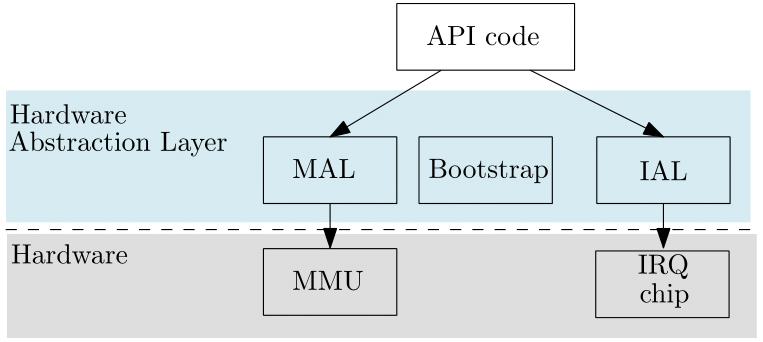
\includegraphics[width=0.58\linewidth,frame]{img/HAL.png} 
	\caption{HAL and API relationship}
	\label{HAL}
\end{figure}

\subsubsection{Formal proofs using Coq} 
\begin{wrapfigure}[6]{r}{0.2\textwidth}
\vspace{-14pt}
\centering

\includegraphics[frame]{img/CoqLogo.png}
\end{wrapfigure}
Coq\cite{Coq} is the result of about 30 years of research.
It started in 1984 as an implementation of the Calculus of Constructions, an expressive formal language, at INRIA by \textit{Thierry Coquand} and \textit{Gérard Huet} and was extended,later in 1991, by Christine to the Calculus of Inductive Constructions. \\

Coq is a \textbf{formal proof management system}. It provides a formal language to write mathematical definitions, executable algorithms and theorems together with an environment for semi-interactive development of machine-checked proofs. Typical applications include the certification of properties of programming languages (e.g. the \textit{CompCert} compiler certification project, or the \textit{Bedrock} verified low-level programming library), the formalization of mathematics (e.g. the full formalization of the Feit-Thompson theorem or homotopy type theory) and teaching. It implements a program specification and mathematical higher-level language called \textit{Gallina} that is based on the Calculus of Inductive Constructions combining both a higher-order logic and a richly-typed functional programming language.\\

As a \textbf{proof development system}, Coq provides interactive proof methods, decision and semi-decision algorithms as well as a tactic language letting the user define his own proof methods. Furthermore, as a \textbf{platform for the formalization of mathematics or the development of programs}, Coq provides support for high-level notations, implicit contents and various other useful kinds of macros.\\

For this project, the latest version of Coq, 8.6 released in December 2016, was used. It features among other things a faster universe checker, asynchronous error processing, proof search improvements, generalized introduction patterns, a new warning system, patterns in abstractions and a new subterm selection algorithm. \\

The Coq proof assistant provides us with powerful tactics to perform proofs. Here is a non exhaustive list of these tactics :
\begin{itemize}
\item \textbf{simpl :} simplifies the current goal;
	\item \textbf{assumption :} solves the current goal if it is computationally equal to a hypothesis;
	\item \textbf{reflexivity :} solves the current goal if it is a valid equality;
	\item \textbf{unfold t :} unfolds the definition of t in the current goal;
	\item \textbf{clear H :} removes hypothesis H from the context;
	\item \textbf{auto :} tries to solve the current goal automatically by using a collection of tactics;
	\item \textbf{rewrite H :} uses an equality hypothesis H to replace a term in the current goal;	
	\item \textbf{induction t:} applies the induction principle for the type of t, generates subgoals as many as there are constructors, and adds the inductive hypotheses in the contexts;
	\item \textbf{inversion H :} resembles the induction tactic, but pays attention to the particular form of the type of H, and will only consider the cases that could have been used, so it discards some impossible cases quickly and efficiently;
	\item \textbf{omega :} carries out an automatic decision procedure for \textit{Presburger} arithmetic;
	\item \textbf{apply H :} mainly tries to unify the current goal with the conclusion of the type of H. If it succeeds, then the tactic returns as many subgoals as non-dependent premises of the type of H;
	\item \textbf{f\_equal :} applies to a goal of the form $f$ a{\tiny 1} \dots a{\tiny n} = $g$ b{\tiny 1} \dots b{\tiny n} and leads to subgoals $f = g$ and a{\tiny 1} = b{\tiny 1} and so on up to a{\tiny n} = b{\tiny n}. Amongst these subgoals, the simple ones are automatically solved;
	\item \textbf{contradiction :} tries to find a contradiction amongst the hypotheses.	
\end{itemize}
Coq also provides several tactics to deal with higher-order logic, particularly targeting binary connectives and quantifiers such as \textbf{split} for conjunction, \textbf{left} and \textbf{right} for disjunction, \textbf{intros} for implication and universal quantifiers and \textbf{exists} for existential quantifiers when they are in the goal. In addition, We have \textbf{destruct} for conjunction and disjunction, \textbf{apply} for implication, \textbf{elim} for existential quantifiers and \textbf{specialize} for universal quantifiers when they are in the hypothesis. Furthermore, many tactics can be preceded with the letter \textit{e} like \textbf{eauto}, \textbf{eassumption} and \textbf{eapply} to deal with existential variables. Some tactics can also be applied on hypotheses if we use the reserved clause \textit{in} with the name of the hypothesis such as unfold, apply and simpl. 
%ref Curry , In throry, \textbf{proving is the same as programming}. 

\subsection{In-depth understanding of PIP's Data structures} \label{structures}

\subsubsection{The memory}

PIP uses several data structures per partition, which will represent the global state of the partition's memory state. This is necessary as it has to keep track of pages allocated to partitions in order to allow or deny derivation and partition creation while preserving the required properties. \\

Figure \ref{partitionEx} shows a partition tree example consisting of a partition, Parent, that has a single child, Child1. A partition is identified by a partition descriptor which is a page number essential to access the whole data structure of a partition. In our case, the partition descriptors of Parent and Child1 are respectively 1 and 12. The pages lent to PIP to manage a partition are organized in a tree with three branches : the MMU tables, the first shadow and the second shadow. The aim of this organization is to keep additional information about each page lent to a partition. Moreover these structures have multiple goals :
\begin{itemize}
	\item \textbf{Access control :} the first shadow is used to avoid deriving the same page multiple times;
	\item \textbf{Performance :} the second shadow and the configuration list are used to quickly find the virtual address of a page without having to parse the whole virtual space when the parent partition reclaims it.
\end{itemize} 
As such, adding an indirection table in the MMU configuration requires two additional pages for the shadows. Therefore, this model is estimated to require roughly three times the amount of memory a simple virtual environment would need, nevertheless it provides a  secure and an efficient API. \\

To prove the isolation properties on this memory structure it is essential to assure its consistency relative to the partition tree, the well-typedness as well as some other consistency properties that will be detailed in section \ref{Hoare} p.\pageref{Hoare}.

\vfill 

\begin{figure}[!ht]  
	\centering 
	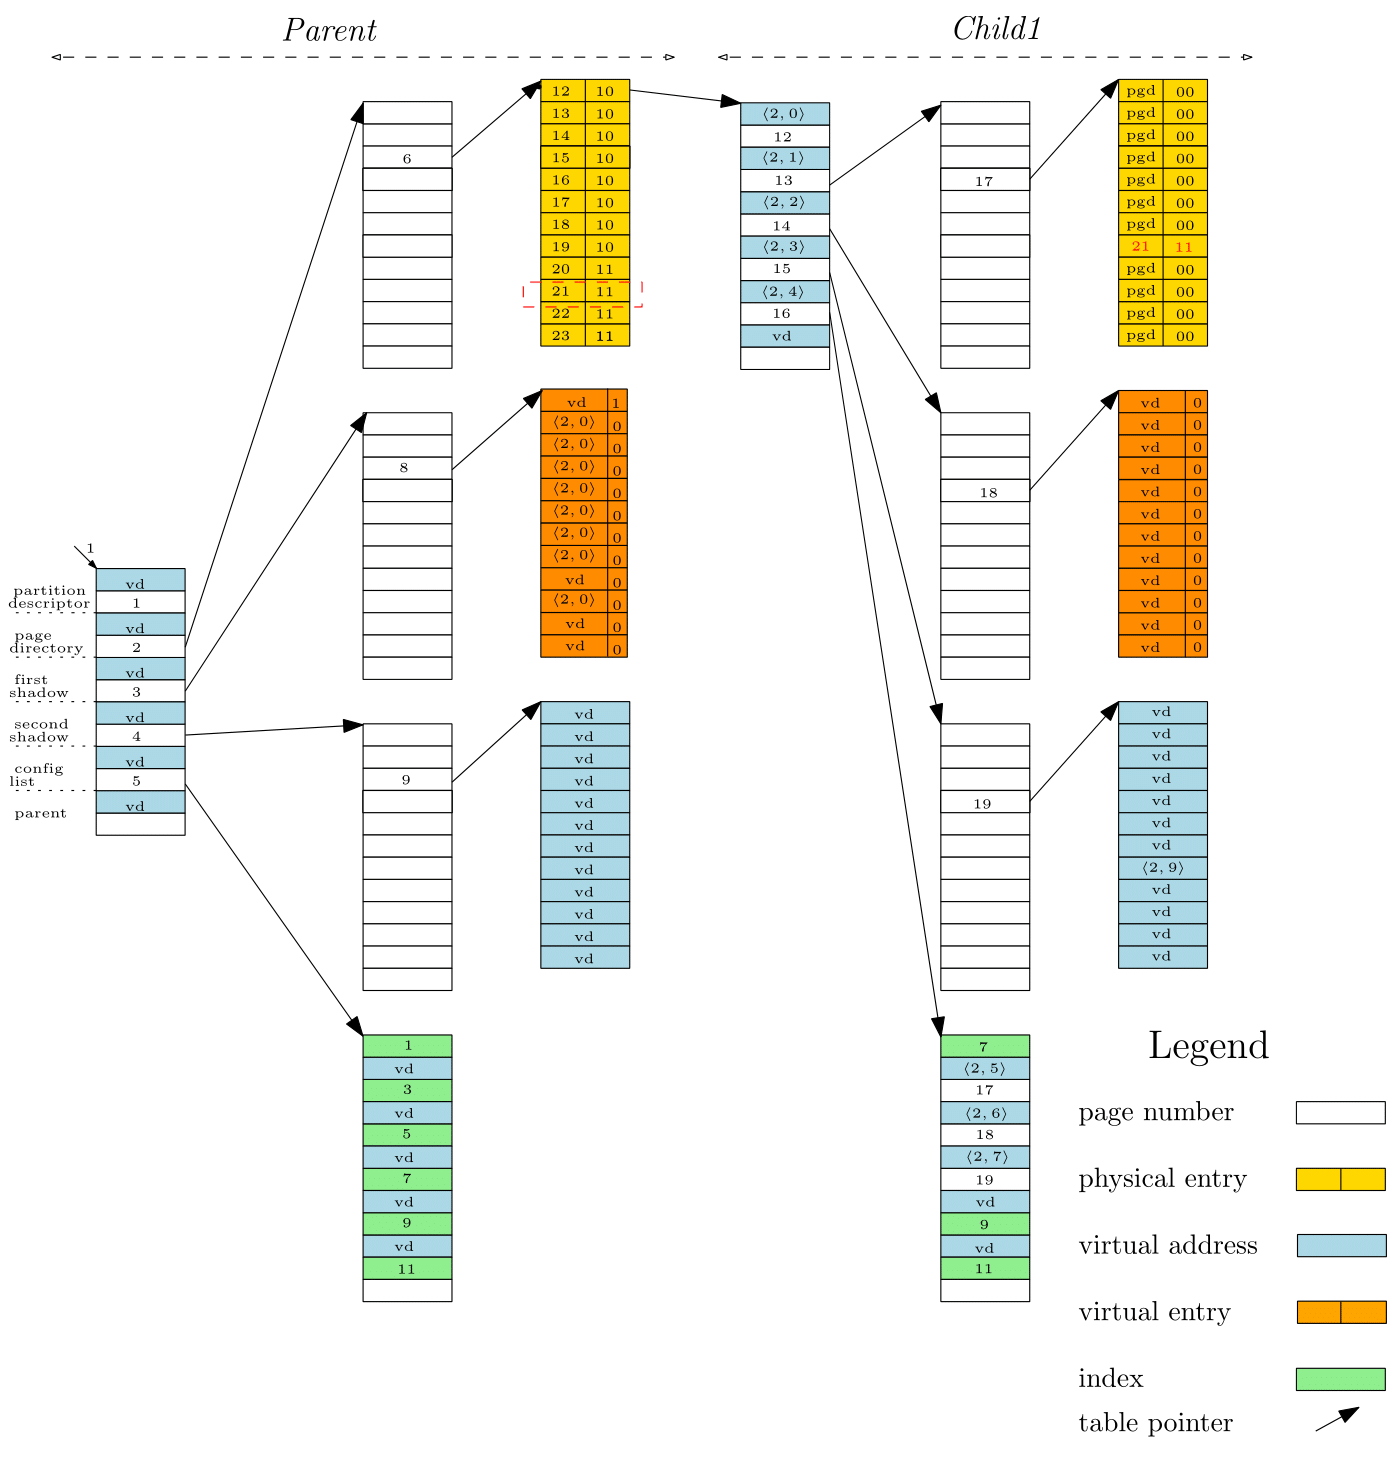
\includegraphics[width=1\linewidth, height=0.6\textheight, frame]{img/memoryEx.png} 
	\caption{An example of a partition tree}
	\label{partitionEx}
\end{figure}

\subsubsection{The state} \label{PIPstateSection}
 
\noindent The PIP state is defined as follows :
\begin{lstlisting}[linewidth=1.02\linewidth,caption = {PIP state definition},label={PIPstate}] 
Record state : Type := 
{ currentPartition: page ; memory: list (paddr * value) }.
\end{lstlisting}
The list in the state corresponds to the physical memory and maps physical addresses to values. A physical address is defined by a physical page number and a position into this page :
\begin{lstlisting}[caption = {paddr type definition},xleftmargin=.15\textwidth,xrightmargin=.15\textwidth] 
Definition paddr : Type := page * index.
\end{lstlisting}
where pages and indexes are positive integers bounded respectively by the overall number of pages and the table size :
\begin{lstlisting}[caption = {page \& index type definitions},xleftmargin=.05\textwidth,xrightmargin=.05\textwidth]
Record page := { p :> nat ; Hp : p < nbPage }. 
Record index := { i :> nat ;  Hi : i < tableSize }.
\end{lstlisting}
Different types of values could be stored in the physical memory by Pip. So, the type \textit{value} is an inductive type defined as follows :
\begin{lstlisting}[caption = {value type definition}, mathescape=true,xleftmargin=.23\textwidth,
xrightmargin=.23\textwidth]
Inductive value : Type :=
	| PE: Pentry $\rightarrow$ value
	| VE: Ventry $\rightarrow$ value
	| PP: page   $\rightarrow$ value
	| VA: vaddr  $\rightarrow$ value
	| I:  index  $\rightarrow$ value.
\end{lstlisting}
The type \textit{Pentry}, which represents a physical entry, consists of a physical page number along with several flags :
\begin{lstlisting}[caption = {Pentry type definition},xleftmargin=.27\textwidth,
xrightmargin=.27\textwidth]
Record Pentry : Type := {
  	read:    bool ;
   	write:   bool ;
   	exec:    bool ;
   	present: bool ;
   	user:    bool ;
   	pa:      page }.
\end{lstlisting}
Finally, the \textit{Ventry} type consists of a virtual address with a unique boolean flag :
\begin{lstlisting}[caption = {Ventry type definition},xleftmargin=.06\textwidth,xrightmargin=.06\textwidth]
Record Ventry : Type := { pd: bool ; va: vaddr }.
\end{lstlisting}
with virtual addresses modelled as a list of indexes of length the number of levels of the MMU plus one :
\begin{lstlisting}[caption = {vaddr type definition},xleftmargin=.02\textwidth,xrightmargin=.02\textwidth]
Record vaddr : Type := 
{ va :> list index ; Hva : length va = nbLevel + 1  }.
\end{lstlisting}

\section{Hoare logic}

\subsection{Introduction to Hoare logic theory} \label{HoareIntro}
\textit{How can we argue that a program is correct ?}
Nowadays, Building reliable software is becoming more and more difficult considering the growing scale, specifications and complexity of modern systems. Therefore, tests alone can no longer ascertain the reliability of programs especially if we're talking about critical systems. Logicians, computer scientists and software engineers have responded to these challenges by developing different kinds of techniques some of which are based on formal reasoning about properties of software and tools for helping validate these properties. One of these reasoning techniques that was used to prove PIP's properties is \textit{Floyd–Hoare logic}, often shortened to just \textbf{Hoare Logic}. It was proposed in 1969 by the British computer scientist and logician Tony Hoare and it continues to be the subject of intensive research right up to the present day. It is not only a natural way of \textbf{writing down specifications of programs} but also a technique for \textbf{proving that programs are correct} with respect to such specifications.\\ % other technique : Model checking

Let S be a program that we want to execute starting from a certain state s, P a predicate on the state describing the condition S relies on for correct execution and Q a predicate on the resulting state after the execution of S describing the condition S establishes after correctly running. Knowing that P is verified on s, if we prove that Q is verified after the execution of s, we can ascertain that S is partially correct. And by partial correctness of S we mean that S is correct if it terminates. Using standard Hoare logic, only partial correctness can be proven, while termination needs to be proven separately. This triple S, P and Q, written as \textbf{ \{P\} S \{Q\} }, is referred to as a \textbf{Hoare triple}. The assertions P and Q are respectively referred to as the \textbf{precondition} and the \textbf{postcondition}. \\

\noindent For example let's consider simple Hoare triples about an assignment command :
\begin{itemize}
	\item \boldmath$\{X=2\} X:=X+1 \{X=3\}$ : is a valid Hoare triple, that can be easily formally proved in Coq, since the postcondition is verified after the execution of the assign command relatively to the precondition;
	\item \boldmath$\{X=2\} X:=X*2 \{X=3\}$ : is not a valid Hoare triple since the postcondition would not be verified after the execution of the command.
\end{itemize} 
\pagebreak
\noindent Now, let's introduce some facts and rules about Hoare triples :
\begin{enumerate}
\item If an assertion P implies another precondition P' of a valid Hoare triple \{P'\} S \{Q\} then \{P\} S \{Q\} is also a valid Hoare triple. This is referred to as \textbf{weakening the precondition of a Hoare triple} and can be formally defined as follows :
\vspace{-10pt}
\begin{prooftree}
\AxiomC{P $\rightarrow$ P'}
\AxiomC{\{P'\} S \{Q\}}
\RightLabel{\small{Hoare\_weaken}}
\BinaryInfC{\{P\} S \{Q\}}
\end{prooftree}
\item If we can weaken a Hoare triple, we expect it to have a \textbf{weakest precondition}. This notion was introduced by Dijkstra in 1976 and is very important since it enables us to prove total correctness and in particular program termination. Indeed, if a program doesn't terminate, its weakest precondition would be \textit{True} and it would verify any postcondition.
\item If we consider a language containing a \textbf{SKIP instruction} which practically does nothing, we can affirm that this command preserves any property which means :
\vspace{-15pt}
\begin{prooftree}
\AxiomC{}
\RightLabel{\small{Hoare\_skip}}
\UnaryInfC{\{P\} SKIP \{P\}}
\end{prooftree}
\item If we consider a language that allows \textbf{assignments}, in the form of \linebreak \emph{X := a}, then we can conclude that an arbitrary property Q holds after such assignment if we assume Q[X$\rightarrow$a] which means Q with all occurrences of X replaced by a :
\vspace{-10pt}
\begin{prooftree}
\AxiomC{}
\RightLabel{\small{Hoare\_assign}}
\UnaryInfC{\{Q[X$\rightarrow$a]\} X:= a \{Q\}}
\end{prooftree}
\item Generally speaking, every Program is built using \textbf{sequencing} of commands that we will write as C1\textbf{;}C2. Our aim is to prove a Hoare triple on this sequence with P and Q respectively as the precondition and the postcondition. This requires proving that C1 takes any state where P holds to a state where an intermediate assertion I holds and C2 takes any state where I holds to one where Q holds which could be formally stated as :
\vspace{-10pt}
\begin{prooftree}
\AxiomC{\{P\} C1 \{I\}}
\AxiomC{\{I\} C2 \{Q\}}
\RightLabel{\small{Hoare\_seq}}
\BinaryInfC{\{P\} C1\textbf{;}C2 \{Q\}}
\end{prooftree}
\item Finally, let's not forget \textbf{conditional structures} that we can write in the form of \emph{IF B THEN C1 ELSE C2}. To verify a Hoare triple about this instruction with P and Q respectively as the precondition and postcondition, we need to consider both cases where B is evaluated to \textit{true} and \textit{false} and prove that Q holds on the resulting state in each one. We can also disregard a case if there is some sort of contradiction relatively to the property P. This rule can be written as follows :
\vspace{-10pt}
\begin{prooftree}
\AxiomC{\{P $\bigwedge$ B\} C1 \{Q\}}
\AxiomC{\{P $\bigwedge \neg$ B\} C2 \{Q\}}
\RightLabel{\small{Hoare\_if}}
\BinaryInfC{\{P\} IF B THEN C1 ELSE C2 \{Q\}}
\end{prooftree}
\end{enumerate}
The rules defined above are in their simplest form and we need to adapt them to the language or semantics we're working on. Also, This list isn't exhaustive\cite{SoftwareFoundation}. For example, we didn't define a rule for \textit{While} loops because the Coq model of PIP doesn't actually use them and uses recursion instead. Likewise, We're sure that all PIP's functions terminate since recursive functions are bounded by a maximum number of iterations.  

\subsection{Hoare logic in the shallow embedding} \label{Hoare}
The Hoare logic devised for the shallow embedding is slightly different from what we saw in the previous section. A program in the shallow embedding is defined in a monadic style that returns a pair of values, the first being the resulting state and the second the value returned by the program which generally corresponds to a function. Thus, as shown in script \ref{shallow_Hoare}, \textbf{the postcondition must not only reason on the resulting state but also on the returned value} so that we can verify it and propagate it in the case of long proofs. The notation chosen for the Hoare triple stays the same as the one mentioned in the previous section except for the brackets that are doubled since single brackets are already used in Coq.
\begin{lstlisting}[caption = {Hoare triple in the shallow embedding},label = {shallow_Hoare}, mathescape=true,xleftmargin=.02\textwidth,
xrightmargin=.02\textwidth]
Definition hoareTriple {A : Type} (P : state $\rightarrow$ Prop) 
(m : LLI A) (Q : A $\rightarrow$ state $\rightarrow$ Prop) : Prop :=
  $\forall$ s, P s $\rightarrow$ match (m s) with
    | val (a, s') => Q a s'
    | undef _ _=> False
    end.

Notation "{{ P }} m {{ Q }}" := (hoareTriple P m Q)
  (at level 90, format "'[' '[' {{  P  }}  ']' '/  '
  '[' m ']' '['  {{  Q  }} ']' ']'") : state_scope.
\end{lstlisting}
The weakening lemma on Hoare triples was also defined and proven as shown in script \ref{shallow_weaken}. This Lemma is extensively used in PIP's proofs.
\begin{lstlisting}[caption = {Weakening Hoare triples in the shallow embedding},label = {shallow_weaken}, mathescape=true,xleftmargin=.06\textwidth,
xrightmargin=.06\textwidth]
Lemma weaken (A : Type) (m : LLI A) 
(P Q : state $\rightarrow$ Prop) (R : A $\rightarrow$ state $\rightarrow$ Prop) :
  {{ Q }} m {{ R }} $\rightarrow$ 
  ($\forall$ s, P s $\rightarrow$ Q s) $\rightarrow$
  {{ P }} m {{ R }}.
Proof.
intros H1 H2 s H3.
case_eq (m s); [intros [a s'] H4 | intros a H4 ];
apply H2 in H3; apply H1 in H3; 
try rewrite H4 in H3; trivial.
intros. rewrite H in H3. assumption. 
Qed.
\end{lstlisting}
Some simple instructions were considered as primitive like conditional structures while some others were explicitly defined, like assignments in the form of \linebreak \textit{\textbf{perform x := m in e}} where the value of the program m gets assigned to x in the evaluation of the program e. Furthermore, a Hoare triple rule was devised for assignments.
\begin{lstlisting}[caption = {Hoare triples assignment rule in the shallow embedding},label = {shallow_assign},mathescape=true]
Lemma bind (A B : Type) (m : LLI A) (f : A $\rightarrow$ LLI B) 
(P : state $\rightarrow$ Prop) ( Q : A $\rightarrow$ state $\rightarrow$ Prop) 
(R : B $\rightarrow$ state $\rightarrow$ Prop) :
  ($\forall$ a, {{ Q a }} f a {{ R }}) $\rightarrow$ 
  {{ P }} m {{ Q }} $\rightarrow$ 
  {{ P }} perform x := m in f x {{ R }}.
Proof. 
intros H1 H2 s H3; unfold bind;
case_eq (m s); [intros [a s'] H4 | intros k s' H4];
apply H2 in H3; rewrite H4 in H3; trivial.
case_eq (f a s'); [intros [b s''] H5 | intros k s'' H5];
apply H1 in H3; rewrite H5 in H3; trivial.
Qed. 
\end{lstlisting}

Finally, to reason with Hoare logic we need to formally  specify the properties we want to prove, the most important being partition memory isolation,
kernel data isolation, vertical sharing and consistency mentioned in \ref{properties} p.\pageref{properties}\cite{MMUIsolation}. To that end, the following necessary functions on PIP's data structures were defined : 
\begin{itemize}
	\item \textbf{getChildren :} returns the list of all children of a given parent partition in the partition tree of a given state;
	\item \textbf{getAncestors :} returns the list of all ancestors of a given partition in the partition tree of a given state;
	\item \textbf{getMappedPages :} returns the list of mapped pages of a given partition;
	\item \textbf{getAccessibleMappedPages :} returns the list of all mapped pages, of a given partition, marked as accessible;
	\item \textbf{getUsedPages :} returns the list of all the pages that are used by a given partition including the pages lent to PIP;
		\item \textbf{getConfigPages :} returns the list of configuration pages lent to PIP to manage a given partition;
	\item \textbf{getPartitions :} returns the list of all existing partitions of a given state which is naturally obtained by a search on the partition tree.
\end{itemize} 
The first property defines horizontal isolation between children i.e., for any state s of the system, all memory pages owned by two different children of a given parent partition in the partition tree must be distinct. This property is formally defined in the Coq proof assistant as follows :
\begin{lstlisting}[caption = {Horizontal isolation}, mathescape=true,xleftmargin=.02\textwidth,
xrightmargin=.02\textwidth]
Definition horizontalIsolation s :=
$\forall$ parent child1 child2,
parent $\in$ getPartitions s $\rightarrow$
child1 $\in$ getChildren parent s $\rightarrow$
child2 $\in$ getChildren parent s $\rightarrow$
child1 $\neq$ child2 $\rightarrow$
(getUsedPages child1 s) $\cap$ (getUsedPages child2 s) = $\emptyset$.
\end{lstlisting}
The second property defines vertical sharing between a parent partition and its children i.e. it ensures that all pages mapped by a child are mapped in its parent. This property is formally defined as follows :
\begin{lstlisting}[caption = {Vertical sharing}, mathescape=true,xleftmargin=.08\textwidth,
xrightmargin=.08\textwidth]
Definition verticalSharing s :=
$\forall$ parent child,
parent $\in$ getPartitions s $\rightarrow$
child $\in$ getChildren parent s $\rightarrow$
getUsedPages child s $\subseteq$ getMappedPages parent s.
\end{lstlisting}
The third property defines kernel data isolation meaning it ensures that for any state of the system and any given two possibly-equal partitions, the code running in the second partition cannot access the pages containing configuration tables lent to PIP to manage the first partition. This property is formally defined as follows :
\begin{lstlisting}[caption = {Kernel data isolation}, mathescape=true,xleftmargin=.12\textwidth,
xrightmargin=.12\textwidth]
Definition kernelDataIsolation s :=
$\forall$ partition1 partition2,
partition1 $\in$ getPartitions s $\rightarrow$
partition2 $\in$ getPartitions s $\rightarrow$
(getAccessibleMappedPages partition1 s) $\cap$
(getConfigPages partition2 s) = $\emptyset$.
\end{lstlisting}
The last property of consistency is mandatory to prove the previously detailed properties. Consistency encompasses different sub-properties that were divided into four categories. As the definition of this property is quite cumbersome, we will only disclose these categories and illustrate each one with an example :
\begin{itemize}
	\item \textbf{Partition tree structure :} the properties in this category ensure that the partition tree of a given state is consistent relatively to its awaited structure preset in section \ref{structures} p.\pageref{structures}. For example, one of the properties defined in this category and called \textit{noCycleInPartitionTree} ensures that there is no cycle in the partition tree of a given system i.e. each partition is different from all its ancestors in the partition tree. This property is formally defined as follows :
\begin{lstlisting}[caption = {Example of partition-tree-consistency property}, mathescape=true,xleftmargin=.08\textwidth,
xrightmargin=.14\textwidth]
Definition noCycleInPartitionTree s :=
$\forall$ ancestor partition,
partition $\in$ getPartitions s $\rightarrow$
ancestor $\in$ getAncestors partition s $\rightarrow$
ancestor $\neq$ partition.
\end{lstlisting}
	\item \textbf{Flag semantics :} This category focuses on the signification of flags used in the data structures. For instance, a property called \textit{isPresentNotDefaultIff} states that the associated page number of a physical entry whose \textit{present} flag is set to \textit{false}, corresponds to the predefined default page value. This property is formally defined as shown in script \ref{flags} where \textit{readPhyEntry} and \textit{readPresent} are predefined functions that respectively read, for a given table, index and memory state, the present flag of a physical entry and its value  :
\begin{lstlisting}[caption = {Example of a flags-semantics-consistency property}, mathescape=true , label={flags}]
Definition isPresentNotDefaultIff s :=
$\forall$ table idx,
readPresent table idx (s.memory) = Some false $\leftrightarrow$
readPhyEntry table idx (s.memory) = Some defaultPage.
\end{lstlisting}	 
	\item \textbf{Pages properties :} This category concerns several properties about the partitions' mapped pages, the pages lent to the kernel as well as the relations between them. For example, the \textit{noDupMappedPagesList} requires that the mapped pages of partitions be distinct from each other, using the function \textit{NoDup} which verifies whether a list contains duplicates or not. This property is formally defined as follows  :
\begin{lstlisting}[caption = {Example of a pages-consistency property}, mathescape=true,xleftmargin=.07\textwidth,
xrightmargin=.07\textwidth]
Definition noDupMappedPagesList s :=
$\forall$ partition, partition $\in$ getPartitions s $\rightarrow$
NoDup (getMappedPages partition s).
\end{lstlisting}	
	\item \textbf{Well-typedness :} This last category concerns kernel data types and ensures that PIP doesn't contain any type confusion. For instance, when PIP writes a virtual address in the memory, it should be read later as a virtual address which is ensured by a property called \textit{dataStructurePdSh1Sh2asRoot}. Otherwise, it is considered as an undefined behaviour in the model.
\end{itemize}
The only Hoare triple that was sucessfully proven to this date\footnotemark[1] is the one about the \textit{createPartition} call that required about 60000 lines of code to prove and which is defined as follows :
\begin{lstlisting}[caption = {createPartition Hoare triple}, mathescape=true]
Lemma createPartition (descChild pdChild
           shadow1 shadow2 list : vaddr) :
{{fun s $\Rightarrow$ partitionsIsolation s  $\bigwedge$ kernelDataIsolation s 
	   $\bigwedge$ verticalSharing s $\bigwedge$ consistency s }} 
createPartition descChild pdChild shadow1 shadow2 list  
{{fun _ s  $\Rightarrow$ partitionsIsolation s $\bigwedge$ kernelDataIsolation 
              s $\bigwedge$ verticalSharing s $\bigwedge$ consistency s }}.
\end{lstlisting}	
\footnotetext[1]{\today}
\pagebreak

\section{The deep embedding} \label{deep}

\subsection{DEC}
DEC\cite{DEC} (Deep Embedding of a
terminating C-style language with effects) is a \gls{DSL} embedded in \textit{Gallina} and developed as an intermediate language for
the translation of PIP to C. DEC Relies on Coq modules to define parametrisable state and identifiers types which are both specified in a module type (\textit{IdModType} defined in annex \ref{ModType} p.\pageref{ModType}). The dynamic semantics of DEC is specified in the style of Structural Operational Semantics\cite{SOS} (SOS) which formally describe how the individual steps of a computation take place enabling us to perform software verification by reasoning on formulas' structure. The DEC language has the following properties : 
\begin{enumerate}
	\item \textbf{Type soundness :} no well-typed program gets stuck on a
non-value, and when a well-typed program terminates it gives a value
of the right type;
	\item \textbf{Termination :} every execution of a well-typed program
ends with a value;
	\item \textbf{Subject reduction :} the execution of a well-typed
program preserves its type at each step ;
	\item \textbf{Deterministic  :} given an initial state, each well-typed
program can only evaluate to one value and one new state;
	\item \textbf{Strong typedness :} each program has at most one
type ;	
\end{enumerate}
DEC supports Hoare logic reasoning, providing proven Hoare logic rules that will be detailed in section \ref{HoareDeepSec} p.\pageref{HoareDeepSec}.

\iffalse
A deep embedding is mainly an \textbf{abstract representation of a language by modelling its expressions as data}. Strictly speaking, The main difference between a shallow and deep embedding is that the former is \textbf{ extensible with regards to adding language constructs} while the latter is \textbf{extensible with regards to adding interpretations of its abstract data types}. A typical approach in PIP's case would have been reasoning on a predefined deep embedding as structural abstraction enables us to perform cost-effective software verification by inversion on formulas' structure. However, defining such an abstract language, at the beginning, is quite tedious and rather intricate since we need to worry about the wingspan of such language and expression soundness among others. Therefore, the tasks of proof engineering and developing the deep embedding were separated. At first, a formal reasoning system based on Hoare logic was built on the shallow embedding as shown in section \ref{Hoare} p.\pageref{Hoare}. Then, an abstract representation of the shallow model was written in \textit{Gallina} which corresponds to the deep embedding. Needless to say, at some point later on, we need to worry about the preservation of proven properties between both embeddings either by proving that there is a bijection between them or by rewriting all the proofs in the deep embedding. By and large, we need to \textbf{ascertain the feasibility of such proofs in the deep embedding} as well as \textbf{compare examples of conducted proofs in both embeddings}.
\fi

\subsection{Deep embedding constructs}
Before we move on to the main constructs of the deep embedding, we need to introduce essential background types and structures :
\begin{itemize}
	\item \textbf{Id type :} represents the identifiers' type in the deep embedding. Typically, identifiers of variables are strings but we can use any other type;
	\item \textbf{Value type :} represents the actual values the programs will be manipulating. They can be built using the constructor \textit{cst} followed by a shallow type and a value that should be of that type. The value type and its constructor are defined as follows :
\vfill
\begin{lstlisting}[caption = {Values in the deep embedding},xleftmargin=.02\textwidth,xrightmargin=.02\textwidth]
(** the internal type of values,
	 parametrised by a semantic type *)
Inductive ValueI (T: Type) : Type := Cst (v: T).

(** the external type of values,
	 hiding the semantic type *)
Definition Value : Type := sigT ValueI.

(** smart value constructor *)
Definition cst (T: Type) (v: T) : Value :=
           @existT Type ValueI T (Cst T v).
\end{lstlisting}
	\item \textbf{QValue type :} represents head normal forms for expressions (here called quasi-values) in the deep embedding which can be either actual values lifted to quasi-values using the constructor \textit{QV} or identifiers of variables in the variable environment that we lift to quasi-functions using the constructor \textit{Var}, as shown in the following script :
\begin{lstlisting}[caption = {Quasi-values in the deep embedding},xleftmargin=.08\textwidth,
xrightmargin=.1\textwidth]
Inductive QValue : Type := Var (x: Id) 
	                 | QV (v: Value).
\end{lstlisting}
	\item \textbf{Fun type :} represents functions in the deep embedding. The definition of this type is detailed in script \ref{Fun} where :
	\begin{itemize}
		\item \textbf{\textit{fenv}} corresponds to the function environment which maps identifiers to functions;
		\item \textbf{\textit{tenv}} corresponds to the typing environment for parameters which maps identifiers to value types;
		\item \textbf{\textit{e0}} and \textbf{\textit{e1}} are expressions in the deep embedding corresponding respectively to the base case and step case;
		\item \textbf{\textit{x}} corresponds to the name of the function;
		\item \textbf{\textit{n}} is the bound. If its value is 0, the first expression \textit{e0} is evaluated else the second expression \textit{e1} gets evaluated. This enables us to define terminating recursive functions.
\vfill
\begin{lstlisting}[caption = {Functions in the deep embedding},label={Fun},xleftmargin=.08\textwidth,
xrightmargin=.22\textwidth]
Inductive Fun : Type :=
	FC (fenv: Envr Id Fun) 
	   (tenv: valTC)
	   (e0 e1: Exp)
	   (x: Id)
	   (n: nat).
\end{lstlisting}
	\end{itemize}
	\item \textbf{QFun type :} represents quasi-functions in the deep embedding which can be either actual functions that we lift to quasi-functions using the constructor \textit{QF} or identifiers of functions in the function environment that we lift to quasi-functions using the constructor \textit{FVar}, as shown in the following script :
\begin{lstlisting}[caption = {Quasi-functions in the deep embedding},xleftmargin=.08\textwidth,
xrightmargin=.14\textwidth]
Inductive QFun : Type := FVar (x: Id) 
	               | QF (f: Fun).
\end{lstlisting}
	\item \textbf{XFun type :} represents generic effects (external stateful functions) in the deep embedding used to define prospective operations on the state and/or an input. It is used by the \textit{Modify} construct of the deep embedding defined in script \ref{DeepEmb} p.\pageref{DeepEmb}, when we want to read the state or perform changes on it and also when we need to implement non-recursive functions. As shown in script \ref{XFun}, it requires an input type \textit{T1} as well as an output type \textit{T2}. Thus, to define state operations, we will mainly need generic effects with \textit{unit} as the input and output type. Moreover, when specifying a generic effect, we only need to worry about the b\_mod attribute as b\_exec and b\_eval are already preset to build respectively the resulting state and value. This implementation deals with the issue of construct extensibility since it enables us to add shallow constructs and even use shallow functions :
\begin{lstlisting}[caption = {generic effects in the deep embedding}, label={XFun}, mathescape=true,xleftmargin=.02\textwidth,
xrightmargin=.02\textwidth]
Record XFun (T1 T2: Type) : Type := {
    b_mod : W $\rightarrow$ T1 $\rightarrow$ prod W T2 ;
    b_exec : W $\rightarrow$ T1 $\rightarrow$ W := 
     fun state input $\Rightarrow$ fst (b_mod state input) ;
    b_eval : W $\rightarrow$ T1 $\rightarrow$ T2 := 
     fun state input $\Rightarrow$ snd (b_mod state input) 
}.       
\end{lstlisting}
\end{itemize}

As shown in script \ref{DeepEmb}, The deep embedding provides us with 8 constructs to build expressions :
\begin{enumerate}
	\item \textbf{Val} \textit{v} \textbf{:} lifts the value \textit{v} to an expression using the constructor \textit{Val};
	\item \textbf{BindN} \textit{e1 e2} \textbf{:} represents a \textbf{sequence} of instructions where the expression \textit{e1} is evaluated first then \textit{e2} next. It is equivalent to ``\textit{e1;;e2}'' in the shallow embedding;
	\item \textbf{BindS} \textit{x e1 e2} \textbf{:} represents an \textbf{assignment}. It is equivalent to ``\textit{perform x := e1 in e2}'' in the shallow embedding. More precisely, the expression \textit{e2} is evaluated in the updated variable environment where \textit{x} gets mapped to the resulting value of the evaluation of \textit{e1};
	\item \textbf{BindMS} \textit{fenv env e} \textbf{:} evaluates the expression \textit{e} in the function environment \textit{fenv} and variable environment \textit{env};
	\item \textbf{IfThenElse} \textit{e1 e2 e3} \textbf{:} represents a \textbf{conditional structure}. It is equivalent to ``\textit{if e1 then e2 else e3}'' in the shallow embedding. This expression is considered well-typed only when \textit{e1} gets evaluated to a deep boolean value;
	\item \textbf{Return} \textit{G qv} \textbf{:} lifts the quasi-value \textit{qv} to an expression using the constructor \textit{Return}. If \textit{qv} is a variable, it gets evaluated in the variable environment. \textit{G} is a flag which affirms whether the construct should get translated to an actual return in C or not. The type \textit{Tag} of \textit{G} is defined as follows :
\begin{lstlisting}[caption = {Tag type in the deep embedding},xleftmargin=.12\textwidth,
xrightmargin=.18\textwidth]
Inductive Tag : Type := LL | RR.      
\end{lstlisting}
	\item \textbf{Apply} \textit{qf ps} \textbf{:} represents \textbf{function application}. If \textit{qf} is a variable it gets evaluated in the function environment. \textit{ps} is the list of parameters which are expressions. They should be well-typed relatively to the typing environment of the function i.e. the resulting value of the evaluation of each parameter's expression should match its awaited type preset in the typing environment. The type \textit{Prms} of \textit{ps} is defined as follows :
\begin{lstlisting}[caption = {Function parameters in the deep embedding},xleftmargin=.05\textwidth,
xrightmargin=.12\textwidth]
Inductive Prms : Type := PS (es: list Exp).     
\end{lstlisting}	
\pagebreak
	\item \textbf{Modify} \textit{T1 T2 VT1 VT2 xf qv} \textbf{:} is used to define affectful state operations and functions. \textit{xf} is the generic effect that specifies the operation, \textit{T1} and \textit{T2} are respectively its input and output types and \textit{VT1} and \textit{VT2} assure that \textit{T1} and \textit{T2} are admissible value types. If \textit{qv} is a variable it gets evaluated in the variable environment. For instance, we can define a simple \textit{SKIP} instruction with the \textit{Modify} construct as follows :
\begin{lstlisting}[caption = {SKIP instruction in the deep embedding},xleftmargin=.02\textwidth,
xrightmargin=.02\textwidth]
Definition xf_skip : XFun unit unit := {|
        b_mod := fun state input => (state,tt) |}.
        
Definition SKIP : Exp := Modify unit unit 
   UnitVT UnitVT xf_skip (QV(cst unit tt))
\end{lstlisting}
\end{enumerate}
More examples of these constructs will be detailed in section \ref{Work} p.\pageref{Work}.
\begin{lstlisting}[caption = {Deep embedding expressions}, label={DeepEmb}]
Inductive Exp : Type :=
 | Val (v: Value)
 | BindN (e1: Exp) (e2: Exp) 
 | BindS (x: Id) (e1: Exp) (e2: Exp)
 | BindMS (fenv: Envr Id Fun) (env: valEnv) (e: Exp)
 | IfThenElse (e1: Exp) (e2: Exp) (e3: Exp) 
 | Return (G: Tag) (qv: QValue)
 | Apply (qf: QFun) (ps: Prms) 
 | Modify (T1 T2: Type) (VT1: ValTyp T1) (VT2: ValTyp T2)
 		(xf: XFun T1 T2) (qv: QValue)
\end{lstlisting}

The deep expressions are meant to be evaluated in certain variable and function environments. To that end, single and multi-step evaluation were defined as follows :
\begin{itemize}
	\item \textbf{EStep fenv env (Conf Exp n e) (Conf Exp n' e') :} represents a \textbf{single-step evaluation} of the expression \textit{e}, in the function environment \textit{fenv} and variable environment \textit{env}, with \textit{n} as the current state. The constructor \textit{Conf} builds a configuration of the type we seek to evaluate which, in our case, is \textit{Exp} and contains the current state as well as the starting expression. \textit{n'} and \textit{e'} are respectively the resulting state and expression. For example, we can affirm that forall function environment \textit{fenv}, variable environment \textit{env}, state \textit{n} and value \textit{v} :
\begin{center}
\textbf{EStep} fenv env (\textbf{Conf} Exp n (Val v)) (\textbf{Conf} Exp n (Val v))
\end{center}

\item \textbf{PrmsStep fenv env (Conf Prms n es) (Conf Prms n' es') :} represents a single-step evaluation of the list of parameters \textit{es} which conducts a single-step evaluation of the first expression in the list. If the first expression is a value, it moves on to the
next parameter;
\item \textbf{EClosure fenv env (Conf Exp n e) (Conf Exp n' e') :} represents a \textbf{multi-step evaluation} of the expression \textit{e} which is defined as a reflexive transitive closure. It uses the predefined single evaluation steps. It is important to note that there exists a state where any expression gets evaluated to a certain value which we conclude from the termination property of the deep embedding. Furthermore, since the evaluation process is deterministic, an expression gets evaluated to a unique value;
\item \textbf{PrmsClosure fenv env (Conf Prms n es) (Conf Exp n' es') :} represents a multi-step evaluation of the list of parameters \textit{es} which conducts a multi-step evaluation of each expression in the list.
\end{itemize}

Finally, the state in the deep embedding is represented with a type parameter \textit{W}, as shown in script \ref{XFun} p.\pageref{XFun}, that can be specified as required. 

\subsection{Hoare logic in the deep embedding} \label{HoareDeepSec}
A Hoare triple in the deep embedding is slightly different from its counterpart in the shallow embedding. Indeed, this new version of the Hoare triple depends on the function environment as well as the variable environment we're evaluating the expression in. Both will be passed to the Hoare triple as parameters along with the expression, the precondition and the postcondition. The precondition is a predicate on the state while the postcondition is a predicate on both the resulting value and state. We must also ensure that the expression we are dealing with is well-typed. Therefore, as shown in script \ref{HoareEval}, a Hoare triple is considered valid if and only if the expression \emph{e} is well-typed and there is an \textit{EClosure} from a certain starting state verifying the precondition to a certain resulting state and value that verify the postcondition with \textit{e} evaluated in the given function and variable environments \textit{fenv} and \textit{env}. \textbf{\{\{P\}\} fenv $>>$ env $>>$ e \{\{Q\}\}} is the chosen notation for the Hoare triple in the deep embedding where \textit{P}, \textit{Q}, \textit{e}, \textit{fenv}, and \textit{env} are respectively the precondition, the postcondition, the expression, the function environment and the variable environment. Furthermore, as the evaluation of parameters is different from that of expressions, we need to devise a separate Hoare triple for parameters as shown in script \ref{HoarePrmsEval} where \textit{EClosure} is replaced by \textit{PrmsClosure}.
\pagebreak
\begin{lstlisting}[caption = {Hoare triple for expressions in the deep embedding}, label={HoareEval},mathescape=true]
Definition THoareTriple_Eval
    (P : W -> Prop) (Q : Value $\rightarrow$ W $\rightarrow$ Prop)
    (fenv: funEnv) (env: valEnv) (e: Exp) : Prop :=
 $\forall$ (ftenv: funTC) (tenv: valTC) 
   (k1: FEnvTyping fenv ftenv)
   (k2: EnvTyping env tenv)
   (t: VTyp)
   (k3: ExpTyping ftenv tenv fenv e t) 
   (s s': W) (v: Value),
 EClosure fenv env (Conf Exp s e) (Conf Exp s' (Val v)) 
 $\rightarrow$ P s $\rightarrow$ Q v s'.
 
Notation "{{ P }} fenv >> env >> e {{ Q }}" := 
(THoareTriple_Eval P Q fenv env e) (at level 90).
\end{lstlisting}
\begin{lstlisting}[caption = {Hoare triple for parameters in the deep embedding}, label={HoarePrmsEval},mathescape=true]
Definition THoarePrmsTriple_Eval
    (P : W $\rightarrow$ Prop) (Q : list Value $\rightarrow$ W $\rightarrow$ Prop)
    (fenv: funEnv) (env: valEnv) (ps: Prms) : Prop :=
 $\forall$ (ftenv: funTC) (tenv: valTC) 
   (k1: FEnvTyping fenv ftenv)
   (k2: EnvTyping env tenv)
   (pt: PTyp)
   (k3: PrmsTyping ftenv tenv fenv ps pt)
   (s s': W) (vs: list Value),
 PrmsClosure fenv env (Conf Prms s ps) (Conf Prms s' 
        (PS (map Val vs))) $\rightarrow$ P s $\rightarrow$ Q vs s'.
\end{lstlisting}

Several Hoare triple rules were devised and proven. We show the importance of these rules in section \ref{HoareRules} p.\pageref{HoareRules}. For simplicity's sake, We will only give the formal definition of some of these rules and not their actual implementation in Coq :
\begin{itemize}
	\item \textbf{weakening lemmas :} the weakening lemma on expressions is the same as the one defined for the shallow embedding in script \ref{shallow_weaken} p.\pageref{shallow_weaken}. However, we need another weakening lemma for a Hoare triple on parameters. The weakest preconditions for expression and parameter triples were also defined as functions called respectively \textit{wp} and \textit{wpPrms}. The two weakening lemmas are formally defined as follows :
\begin{prooftree}
\AxiomC{\{\{P'\}\} fenv $>>$ env $>>$ e \{\{Q\}\}}
\AxiomC{P $\rightarrow$ P'}
\RightLabel{\small{weakenEval}}
\BinaryInfC{\{\{P\}\} fenv $>>$ env $>>$ e \{\{Q\}\}}
\end{prooftree}	
\begin{prooftree}
\AxiomC{THoarePrmsTriple\_Eval P' Q fenv env ps}
\AxiomC{P $\rightarrow$ P'}
\RightLabel{\small{weakenPrms}}
\BinaryInfC{THoarePrmsTriple\_Eval P Q fenv env ps}
\end{prooftree}	
	\item \textbf{BindS rule :} the assignment rule in the deep embedding is quite different from the shallow one, defined in script \ref{shallow_assign} p.\pageref{shallow_assign}, as environments are now explicitly manipulated. Therefore, to prove a Hoare triple on an assignment of the form \textit{BindS x e1 e2}, we need to prove a Hoare triple on \textit{e2} where \textit{x} is mapped to the resulting value of \textit{e1} in the updated variable environment. To that end, we need an intermediate predicate that will ascertain the validity of the resulting value. This rule is formally defined as follows : 
\begin{prooftree}
\AxiomC{\{\{P0\}\} fenv $>>$ env $>>$ e1 \{\{P1\}\}}
\noLine
\UnaryInfC{$\forall$ v, \{\{P1 v\}\} fenv $>>$ (x,v):env $>>$ e2 \{\{P2\}\}}
\RightLabel{\small{BindS\_VHTT1}}
\UnaryInfC{\{\{P0\}\} fenv $>>$ env $>>$ BindS x e1 e2 \{\{P2\}\}}
\end{prooftree}
	 \item \textbf{BindN rule :} a variant of the \textit{Hoare\_seq} rule, introduced in section \ref{HoareIntro} p.\pageref{HoareIntro}, which requires an intermediate predicate to prove a Hoare triple on a sequence of instructions. It is  formally defined as follows : 
\begin{prooftree}
\AxiomC{\{\{P0\}\} fenv $>>$ env $>>$ e1 \{\{fun \_ $\Rightarrow$ P1\}\}}
\noLine
\UnaryInfC{\{\{P1\}\} fenv $>>$ env $>>$ e2 \{\{P2\}\}}
\RightLabel{\small{BindN\_VHTT1}}
\UnaryInfC{\{\{P0\}\} fenv $>>$ env $>>$ BindN e1 e2 \{\{P2\}\}}
\end{prooftree}
	\item \textbf{IfThenElse rule :} a variant of the \textit{Hoare\_if} rule, introduced in section \ref{HoareIntro} p.\pageref{HoareIntro}. In the deep embedding, we need an intermediate predicate to evaluate the condition then we reason on both possible cases. This rule is formally defined as follows :
\vspace{-1em} 
\begin{prooftree}
\AxiomC{\{\{P0\}\} fenv $>>$ env $>>$ e1 \{\{P1\}\}}
\noLine
\UnaryInfC{\{\{P1 (cst bool true)\}\} fenv $>>$ env $>>$ e2 \{\{P2\}\}}
\noLine
\UnaryInfC{\{\{P1 (cst bool false)\}\} fenv $>>$ env $>>$ e3 \{\{P2\}\}}
\RightLabel{\small{IfTheElse\_VHTT1}}
\UnaryInfC{\{\{P0\}\} fenv $>>$ env $>>$ IfThenElse e1 e2 e3 \{\{P2\}\}}
\end{prooftree}
	\item \textbf{Apply rules :} the apply construct has several rules :
	\begin{itemize}
	\item \textbf{Apply\_VHTT1 :} the main rule of the Apply construct which evaluates not only the parameters but also the next recursive call of the function by performing a pattern matching on the bound. It is formally defined in Coq as follows :
\begin{lstlisting}[caption = {Main Hoare triple rule for the Apply construct},mathescape=true,
xleftmargin=-.14\textwidth]
Lemma Apply_VHTT1 (P0: W $\rightarrow$ Prop) 
   (P1: list Value $\rightarrow$ W $\rightarrow$ Prop) 
   (P2: Value $\rightarrow$ W $\rightarrow$ Prop)  
   (fenv: funEnv) (env: valEnv) 
   (f: Fun) (es: list Exp) : 
 THoarePrmsTriple_Eval P0 P1 fenv env (PS es) $\rightarrow$
 match f with
  | FC fenv' tenv' e0 e1 x n $\Rightarrow$ 
    length tenv' = length es /\     
    match n with
    | 0 $\Rightarrow$ ($\forall$ vs: list Value,  
       THoareTriple_Eval (P1 vs) P2 fenv' 
           (mkVEnv tenv' vs) e0)
    | S n' $\Rightarrow$ ($\forall$ vs: list Value,
       THoareTriple_Eval (P1 vs) P2 
           ((x,FC fenv' tenv' e0 e1 x n')::fenv')
           (mkVEnv tenv' vs) e1)
    end
  end $\rightarrow$             
 THoareTriple_Eval P0 P2 fenv env (Apply (QF f) (PS es)).
\end{lstlisting}
		\item \leftskip -4em
 \textbf{Apply\_VHTT2 :} only evaluates the parameters in a function application. It's de defined as follows : 
\vspace{-1em} 
\begin{prooftree}
\leftskip -6em
\AxiomC{THoarePrmsTriple\_Eval P0 P1 fenv env (PS es)}
\noLine
\UnaryInfC{$\forall$ vs, \{\{P1 vs\}\} fenv $>>$ env $>>$ Apply (QF f) (PS (map Val vs)) \{\{P2\}\}}
\RightLabel{\small{Apply\_VHTT2}}
\UnaryInfC{\{\{P0\}\} fenv $>>$ env $>>$ Apply (QF f) (PS es) \{\{P2\}\}}
\end{prooftree}	
\vspace{0.5em} 	
		\item \textbf{QFun\_VHTT :} evaluates a function variable in an \textit{Apply} construct by searching its value in the function environment. It is formally defined as follows :
\vspace{-1em} 
\begin{prooftree}
\AxiomC{findET fenv x f}
\noLine
\UnaryInfC{\{\{P\}\} fenv $>>$ env $>>$ Apply (QF f) (PS es) \{\{Q\}\}}
\RightLabel{\small{QFun\_VHTT}}
\UnaryInfC{\{\{P\}\} fenv $>>$ env $>>$ Apply (FVar x) (PS es) \{\{Q\}\}}
\end{prooftree}	
	\end{itemize}
\end{itemize}
